\documentclass[12pt,aspectratio=169]{beamer}
\input{../../mybeamer}

\title{Classes 11 \& 12: Circuit Analysis, Part 1}
\subtitle{AP Physics C: E\&M}
\input{../../me}
\input{../../mycommands}

\begin{document}

\begin{frame}
  \maketitle
\end{frame}




\section{Electric Current}

\begin{frame}{Electric Current}
  In an electric circuit, a large number of ``charge carriers'' are pushed
  along by a small electrostatic force\footnote{Charge carriers experience an
  electrostatic force because there is an electric field from the positive
  terminal towards the negative terminal.}, creating an
  \textbf{electric current}. We can \emph{model} positive charges moving from
  the positive terminal towards the negative terminal.
  \begin{center}
    \begin{tikzpicture}[scale=.85,thick]
      \fill[gray!20] rectangle (7,3);
      \draw[very thick] (0,0)--(7,0);
      \draw[very thick] (0,3)--(7,3);
      
      \draw[magenta,fill=magenta!10] (1,.5) circle(.25) node{$+$};
      \draw[magenta,thick,axes] (1.25,.5)--(1.75,.5);

      \draw[magenta,fill=magenta!10] (3,.75) circle(.25) node{$+$};
      \draw[magenta,thick,axes] (3.25,.75)--(3.75,.75);

      \draw[magenta,fill=magenta!10] (6,1.75) circle(.25) node{$+$};
      \draw[magenta,thick,axes] (6.25,1.75)--(6.75,1.75);

      \draw[magenta,fill=magenta!10] (5,2.5) circle(.25) node{$+$};
      \draw[magenta,thick,axes] (5.25,2.5)--(5.75,2.5);

      \draw[magenta,fill=magenta!10] (4,1.75) circle(.25) node{$+$};
      \draw[magenta,thick,axes] (4.25,1.75)--(4.75,1.75);

      \draw[magenta,fill=magenta!10] (5.25,1) circle(.25) node{$+$};
      \draw[magenta,thick,axes] (5.5,1)--(6,1);

      \draw[magenta,fill=magenta!10] (2,1.5) circle(.25) node{$+$};
      \draw[magenta,thick,axes] (2.25,1.5)--(2.75,1.5);

      \draw[magenta,fill=magenta!10] (.5,2.5) circle(.25) node{$+$};
      \draw[magenta,thick,axes] (.75,2.5)--(1.25,2.5);

      \draw[magenta,fill=magenta!10] (2.5,2.25) circle(.25) node{$+$};
      \draw[magenta,thick,axes] (2.75,2.25)--(3.25,2.25);

      \node at (0,1.5)[left] {\huge$+$};
      \node at (7,1.5)[right]{\huge$-$};
    \end{tikzpicture}
  \end{center}
  In metal conductors, \textbf{charge carriers} are valence electrons. In other
  situations motions of ions can also generate an electric current.
  \vspace{.2in}
\end{frame}


\begin{frame}{Current}
  The \textbf{electric current} $I(t)$ is defined as the rate at which
  \textbf{charges} $Q$ pass through a point in a circuit. In differential form:
  
  \eq{-.1in}{
    \boxed{I(t)=\diff Qt} = \frac QV\diff Vt = (ne)(Av_d)
  }
  \begin{itemize}
  \item $Q/V$ is the amount of charge carriers \emph{per volume}, which
    is just
    the \textbf{charge carrier density} (number of charge carriers per volume)
    $n$ times the \textbf{elementary charge} $e$
  \item $\diff V/t$ is the rate the volume of charges moves through the
    conductor, give by the wire's cross-section area $A$ times the
    \textbf{drift velocity} $v_d$ of the charge carrier
  \end{itemize}
\end{frame}



\begin{frame}{Charge Carrier Density}
  Calculating the charge carrier density in a \emph{metal} conductor involves
  some physical information about the metal:
  \begin{enumerate}
  \item Divide the metal's density $\rho$ by its molar mass $M$ to find the
    \emph{number of moles of atoms per unit volume}
  \item Multiply by Avogadro's number $N_A=\SI{6.0221e23}{\per\mol}$ to find
    \emph{number of atoms per unit volume}
  \item Multiply by the number of free electrons per atom $k$ for that
    particular metal
  \end{enumerate}
\end{frame}



\begin{frame}{Charge Carrier Density}
  Collecting all the terms from the last slide, we have:
  
  \eq{-.1in}{
    \boxed{n=\frac{\rho kN_A}M}
  }
  \begin{center}
    \begin{tabular}{l|c|c}
      \rowcolor{pink}
      \textbf{Quantity} & \textbf{Symbol} & \textbf{SI Unit} \\ \hline
      Charge carrier density   & $n$    & \si{\per\metre\cubed} \\
      Density of material      & $\rho$ & \si{\kilo\gram\per\metre\cubed} \\
      Free electrons per atom  & $k$    & \\
      Avogadro's number        & $N_A$  & \si{\per\mol}\\
      Molar mass               & $M$    & \si{\kilo\gram\per\mol}
    \end{tabular}
  \end{center}
  For copper, $M=\SI{63.54e-3}{\kilo\gram\per\mol}$,
  $\rho=\SI{8.96e3}{\kilo\gram\per\metre\cubed}$, $k=1$ and therefore
  $n=\SI{8.5e28}{\per\metre\cubed}$. The drift velocity is in the order of
  $v\approx\SI1{\milli\metre\per\second}$.
\end{frame}



\begin{frame}{Direct Current}
  In a \textbf{direct current} (\textbf{DC}), the flow of charges is always in
  the same direction, but the current itself does \emph{not} have to be
  constant in time. Below are all examples of direct currents.
  
  \vspace{-.15in}\begin{columns}[T]
    \column{.33\textwidth}
    \begin{center}
      \begin{tikzpicture}[scale=.7]
        \draw[functions] (0,3)--(4,3);
        \draw[axes] (0,0)--(4,0) node[right]{$t$};
        \draw[axes] (0,0)--(0,4) node[above]{$I$};
      \end{tikzpicture}
    \end{center}
    \vspace{-.1in}{\footnotesize A circuit with only resistors has a constant,
      time-independent current\par
    }
    
    \column{.32\textwidth}
    \begin{center}
      \begin{tikzpicture}[scale=.7]
        \draw[smooth,samples=20,domain=0:3.5,functions]
        plot(\x,{3*(exp(-.8*\x))});
        \draw[axes] (0,0)--(4,0) node[right]{$t$};
        \draw[axes] (0,0)--(0,4) node[above]{$I$};
      \end{tikzpicture}
    \end{center}
    \vspace{-.1in}{\footnotesize A circuit with a charging or discharging
      capacitor has an exponentially decaying current\par}
    
    \column{.32\textwidth}
    \begin{center}
      \begin{tikzpicture}[scale=.7]
        \draw[axes] (0,0)--(4,0) node[right]{$t$};
        \draw[axes] (0,0)--(0,4) node[above]{$I$};
        \draw[smooth,samples=20,domain=0:3.5,functions]
        plot(\x,{sin(120*\x)+2});
      \end{tikzpicture}
    \end{center}
    \vspace{-.1in}{\footnotesize A circuit with capacitors and inductors has a
      current that has a sinusoidal component\par}
  \end{columns}
\end{frame}



\begin{frame}{Alternating Current}
  In contrast, in an \textbf{alternating current} (\textbf{AC}), the flow of
  charges changes in direction, \emph{usually} as a sinusoidal function of time.
  \begin{center}
    \begin{tikzpicture}[scale=.7]
      \draw[smooth,samples=50,domain=0:4,functions] plot(\x,{1.5*sin(150*\x)});
      \draw[axes] (0,0)--(5,0) node[right]{$t$};
      \draw[axes] (0,-2.5)--(0,2.5) node[above]{$I$};
    \end{tikzpicture}
    \begin{tikzpicture}[scale=.7]
      \draw[smooth,samples=50,domain=0:4,functions] plot(\x,{1.5*sin(150*\x)});
      \draw[axes] (0,0)--(5,0) node[right]{$t$};
      \draw[axes] (0,-2.5)--(0,2.5) node[above]{$V$};
    \end{tikzpicture}
  \end{center}
  The power outlet in North America are all AC, with a RMS (root-mean-square)
  voltage of \SI{120}\volt, and a frequency of \SI{60}\hertz.
\end{frame}



\begin{frame}{Current}
  Another alternate description of the electric current is to express it in
  terms of the \textbf{current density} $J$, with a unit of of \emph{amp\`{e}re
    per meters squared} (\si{\ampere\per\meter\squared}).\footnote{We had
    previously encountered this quantity when studying Amp\`{e}re's law.}

  \eq{-.1in}{
    \boxed{I(t)=J(t)A}
  }

  It is obvious from the previous expression that the current density is the
  product of the charge carrier density, elementary charge, and the drift
  velocity:

  \eq{-.1in}{
    \boxed{J=nev_d}
  }
\end{frame}



\begin{frame}{Electric Current in Metal Conductors}
  In metal conductors, atoms are bonded to each other via
  \textbf{metallic bonds}. The atoms are arranged in a lattice-crystalline
  structure, and they share a cloud of valence electrons. Depending on the
  element, each atom may have 1 or 2 ``free electrons'' that can move under a
  very weak electric field inside the material. (This was discussed earlier, in
  Classes \#1 and \#2.)
  \begin{center}
    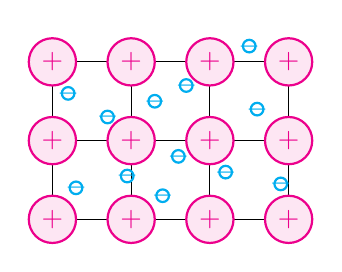
\begin{tikzpicture}
      \draw grid (3,2);
      \foreach \x in {0,...,3}{
        \foreach \y in {0,1,2}
        \draw[thick,magenta,fill=magenta!10] (\x,\y) circle (.3) node{$+$};
      }
      \begin{scope}[thick, cyan,fill=cyan!10]
        \draw (.2,1.6) circle (.08) node{$-$};
        \draw (.7,1.3) circle (.08) node{$-$};
        \draw (1.3,1.5) circle (.08) node{$-$};
        \draw (1.7,1.7) circle (.08) node{$-$};
        \draw (2.5,2.2) circle (.08) node{$-$};
        \draw (2.6,1.4) circle (.08) node{$-$};
        \draw (.3,.4) circle (.08) node{$-$};
        \draw (.95,.55) circle (.08) node{$-$};
        \draw (1.6,.8) circle (.08) node{$-$};
        \draw (1.4,.3) circle (.08) node{$-$};
        \draw (2.2,.6) circle (.08) node{$-$};
        \draw (2.9,.45) circle (.08) node{$-$};
      \end{scope}
    \end{tikzpicture}
  \end{center}
  Materials based on \textbf{ionic} and \textbf{covalent} bonds do not conduct
  electricity because neither have any free electrons.
\end{frame}



\begin{frame}{Electric Current in Metal Conductors}
  \begin{columns}[T]
    \column{.3\textwidth}
    \vspace{-.0in}
    \begin{center}
      Conventional Current
      
      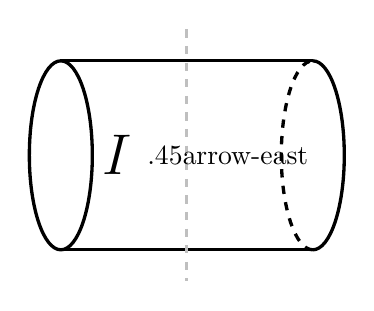
\begin{tikzpicture}[scale=.4]
        \draw[very thick] ellipse (1 and 3);
        \draw[very thick] (0,3)--+(8,0);
        \draw[very thick] (0,-3)--+(8,0);
        \draw[very thick] (8,-3) arc(-90:90:1 and 3);
        \draw[very thick,dashed] (8,-3) arc (270:90:1 and 3);
        \draw[very thick,dashed,lightgray] (4,4)--(4,-4);
        \node at (1.8,0){\huge$I$};
        \node at (5.3,0){\pic{.45}{arrow-east}};
      \end{tikzpicture}
    \end{center}
    \vspace{-.1in}{\scriptsize\textbf{Conventional current} flows from the
      positive terminal (cathode) to the negative terminal (anode). The flow
      of current is assumed to be a continuous function of time\par
    }
    
    \column{.34\textwidth}
    \color{red}\begin{center}
      Model: motion of (+) charges
      
      \begin{tikzpicture}[scale=.4]
        \draw[very thick] ellipse (1 and 3);
        \draw[very thick] (0,3)--+(8,0);
        \draw[very thick] (0,-3)--+(8,0);
        \draw[very thick] (8,-3) arc(-90:90:1 and 3);
        \draw[very thick,dashed] (8,-3) arc (270:90:1 and 3);
        \draw[very thick,dashed,lightgray] (4,4)--(4,-4);
        
        \draw[thick,fill=pink!20] (1.5,1) circle (.4) node{$+$};
        \draw[vectors] (1.9,1)--+(1.5,0);

        \draw[thick,fill=pink!20] (2,-1.3) circle (.4) node{$+$};
        \draw[vectors] (2.4,-1.3)--+(1.5,0);

        \draw[thick,fill=pink!20] (3,1.9) circle (.4) node{$+$};
        \draw[vectors] (3.4,1.9)--+(1.5,0);

        \draw[thick,fill=pink!20] (3.8,0) circle (.4) node{$+$};
        \draw[vectors] (4.2,0)--+(1.5,0) node[right=-2]{\small$\vec F_q$};

        \draw[thick,fill=pink!20] (5.3,-2) circle (.4) node{$+$};
        \draw[vectors] (5.7,-2)--+(1.5,0);

        \draw[thick,fill=pink!20] (6.3,1.5) circle (.4) node{$+$};
        \draw[vectors] (6.7,1.5)--+(1.5,0);
      \end{tikzpicture}
    \end{center}
    \vspace{-.1in}{\scriptsize We assume that positive charge carriers are
      positively charged, and they move with the same \textbf{drift velocity}.
      In most circuits, drift velocity is in the order of 0.1 to
      \SI1{\milli\metre\per\second}.\par}
    
    \column{.32\textwidth}
    \color{blue}
    \begin{center}
      Reality: \textbf{electrons flow}
      \begin{tikzpicture}[scale=.4]
        \draw[very thick] ellipse (1 and 3);
        \draw[very thick] (0,3)--+(8,0);
        \draw[very thick] (0,-3)--+(8,0);
        \draw[very thick] (8,-3) arc(-90:90:1 and 3);
        \draw[very thick,dashed] (8,-3) arc (270:90:1 and 3);
        \draw[very thick,dashed,lightgray] (4,4)--(4,-4);

        \draw[axes] (5,1)--(4,0)--(2.5,.5)--(.5,.8)--(0,0);
        \draw[thick,fill=pink!20] (5,1) circle (.4) node{\small$e^-$};

        \draw[axes] (8,-1)--(5,0)--(4.5,-.5)--(0,-.8); %--(0,0);
        \draw[thick,fill=pink!20] (8,-1) circle (.4) node{\small$e^-$};

        \draw[axes] (6.5,-1.8)--(4.2,-2)--(4,-1)--(2.5,-1.8)--(1,-1.5);
        \draw[thick,fill=pink!20] (6.5,-1.8) circle (.4) node{\small$e^-$};

        \draw[axes] (2.5,1.8)--(0,1.8);
        \draw[thick,fill=pink!20] (2.5,1.8) circle (.4) node{\small$e^-$};
      \end{tikzpicture}
    \end{center}
    \vspace{-.1in}{\scriptsize In reality, electrical current comes from motion
      of negatively-charged electrons in the \emph{opposite} direction of
      convention current. The electron's motion is chaotic, because as they
      move, they collide with other electrons and atoms. Drift velocity is
      the \emph{average} velocity of the electrons\par}
  \end{columns}
  \vspace{.1in}For circuit analysis, we use the conventional current for
  simplicity.
\end{frame}



\begin{frame}{Electric Current in Solutions}
  Materials that are formed by ionic bonds (e.g.\ sodium chloride, or table
  salt) do not conduct electricity, but they can be dissolved (e.g.\ in water)
  and the solution containing the ions is now conductive.
  \begin{center}
    \begin{tikzpicture}
      \draw[fill=cyan!20] rectangle (6,2.5);
      \foreach \x in {.4,5.6} \draw[line width=3] (\x,.5)--(\x,2);
      \draw[thick] (.4,1.25)--+(-1.5,0) node[left]{\large$+$};
      \draw[thick] (5.6,1.25)--+(1.5,0) node[right]{\large$-$};

      \begin{scope}[thick,magenta,fill=magenta!10]
        \draw[vectors] (1.2,2)--+(.5,0); \draw (1,2) circle (.2) node{$+$};
        \draw[vectors] (2.2,1.3)--+(.5,0); \draw (2,1.3) circle (.2) node{$+$};
        \draw[vectors] (3,.4)--+(.5,0); \draw (2.8,.4) circle (.2) node{$+$};
        \draw[vectors] (4.2,1.7)--+(.5,0); \draw (4,1.7) circle (.2) node{$+$};
        \draw[vectors] (3.5,1)--+(.5,0); \draw (3.3,1) circle (.2) node{$+$};
        \draw[vectors] (5,1.3)--+(.5,0); \draw (4.8,1.3) circle (.2) node{$+$};
      \end{scope}
      \begin{scope}[thick,cyan,fill=cyan!10]
        \draw[vectors] (1,1.2)--+(-.5,0);
        \draw (1.2,1.2) circle (.2) node{$-$};

        \draw[vectors] (1.7,.7)--+(-.5,0);
        \draw (1.9,.7) circle (.2) node{$-$};

        \draw[vectors] (2.8,2)--+(-.5,0);
        \draw (3,2) circle (.2) node{$-$};

        \draw[vectors] (3.1,1.6)--+(-.5,0);
        \draw (3.3,1.6) circle (.2) node{$-$};

        \draw[vectors] (4.5,.5)--+(-.5,0);
        \draw (4.7,.5) circle (.2) node{$-$};
      \end{scope}
    \end{tikzpicture}
  \end{center}
  \begin{itemize}
  \item Positive ions move towards negative terminal; while
  \item Negative ions move towards positive terminal
  \end{itemize}
\end{frame}
%
%
%
%\begin{frame}{Electric Current: Conventional vs.\ Electron Flow}
%  The flow of electric current assumes the flow of \emph{positive} charges. We
%  call this the \textbf{conventional current}:
%  \begin{center}
%    \begin{tikzpicture}[scale=.8]
%      \draw (0,0)--(10,0);
%      \draw (0,1)--(10,1) node[midway,above]{$I\longrightarrow$};
%      \foreach \x in {1,3,...,9}{
%        \draw[thick,fill=pink!40] (\x,.5) circle (.25) node{$+$};
%        \draw[vectors] (\x+.25,.5)--(\x+.75,.5);
%      }
%    \end{tikzpicture}
%  \end{center}
%  In a conducting wire, however, negatively charged electrons flow in the
%  opposite direction. We call this the \textbf{electron current}:
%  \begin{center}
%    \begin{tikzpicture}[scale=.8]
%      \draw (0,0)--(10,0);
%      \draw (0,1)--(10,1) node[midway,above]{$I\longrightarrow$};
%      \foreach \x in {1,3,...,9}{
%        \draw[thick,fill=blue!40!gray!20] (\x,.5) circle (.25) node{$-$};
%        \draw[vectors] (\x-.25,.5)--(\x-.75,.5);
%      }
%    \end{tikzpicture}
%  \end{center}
%  %Even though it is actually electron that are moving, we will continue to
%  %treat electric current as the flow of positive charges in the direction of
%  %the conventional current.
%\end{frame}


\begin{frame}{Electric Field Inside the Wire}
  Inside the wire, there is a weak electric field, which exerts a force on the
  free electrons as they move in the wire
  \begin{itemize}
  \item As the charges move through a conductor, they lose potential energy
    (because electric potential is a conservative force)
  \item Unlike a free-falling objects in a vacuum, where gravitational potential
    energy is completely converted into kinetic energy, in a circuit, charge
    carriers do not move in a vacuum, and their potential energy is transformed
    into other forms
  \end{itemize}
\end{frame}



\section{Resistance}

\begin{frame}{Ohm's Law}
  Georg Ohm discovered that when you pass an electric current through a
  conductor, the voltage (electric potential difference) $V$ the two ends of
  the conductor is \emph{linearly proportional} to the amount of current $I$
  through the material
  \begin{center}
    \vspace{-.1in}
    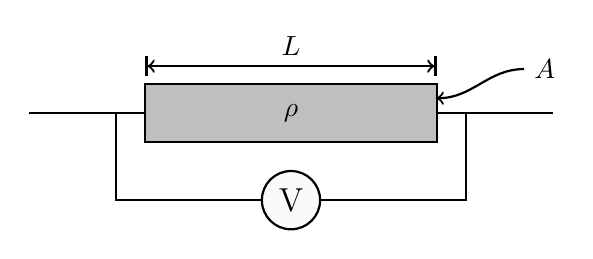
\begin{tikzpicture}[thick,scale=.37]
      \draw (-4,0)--(14,0);
      \draw (-1,0)--(-1,-3)--(11,-3)--(11,0);
      \draw[fill=lightgray] (0,-1) rectangle (10,1) node[midway]{$\rho$};
      \draw[fill=black!2] (5,-3) circle (1) node{\large V};
      \draw[thick,|<->|] (0,1.6)--(10,1.6) node[midway,above]{$L$};
      \draw[thick,<-] (10,.5) to[out=0,in=180] (13,1.5) node[right]{$A$};
    \end{tikzpicture}
  \end{center}
  The proportionality constant between voltage and is called
  \textbf{resistance}. Note that Ohm's law is not a fundamental law in physics.
\end{frame}


\begin{frame}{Ohm's Law}
  \textbf{Ohm's law} relates electric potential difference $V$ across a
  conductor to the amount of current $I$ through the conductor through the
  \textbf{resistance} $R$ of the conductor:

  \eq{-.2in}{
    \boxed{V=IR}
  }
  \begin{center}
    \begin{tabular}{l|c|c}
      \rowcolor{pink}
      \textbf{Quantity} & \textbf{Symbol} & \textbf{SI Unit} \\ \hline
      Potential difference & $V$    & \si\volt \\
      Current              & $I$    & \si\ampere \\
      Resistance           & $R$    & \si\ohm
    \end{tabular}
  \end{center}
  Resistance is due to collisions between the free electrons
  %(which causes the current)
  with the atoms in the conductor.
  \begin{itemize}
  \item The collisions transfer energy from the electrons to the atoms
  \item The additional energy causes the atoms to vibrate
  \item The vibrations causes the atoms to emit \textbf{electromagnetic
    radiation}
  \end{itemize}
\end{frame}


\begin{frame}{Resistance of a Conductor}
  The resistance of a conductor is proportional to the resistivity $\rho$ and
  its length $L$, and inversely proportional to the cross-sectional area $A$:

  \eq{-.1in}{
    \boxed{
      R=\int\dl R=\rho\int_0^L\frac{\dl x}{A(x)}
    }
  }
  \begin{center}
    \begin{tabular}{l|c|c}
      \rowcolor{pink}
      \textbf{Quantity} & \textbf{Symbol} & \textbf{SI Unit} \\ \hline
      Resistance           & $R$    & \si\ohm \\
      Resistivity          & $\rho$ & \si{\ohm\metre} \\
      Length of conductor  & $L$    & \si\metre \\
      Cross-sectional area & $A(x)$ & \si{\metre\squared}
    \end{tabular}
  \end{center}
  The resistivity $\rho$ is determined by the material.\footnote{Don't confuse
  resistivity with the \emph{density} of the material; both use the same Greek
  letter $\rho$} For an ``ohmic'' device, resistivity should be independent of
  temperature and direction of current.
  \vspace{.2in}
\end{frame}


\begin{frame}{Resistance of a Conductor}
  For a resistor with constant cross sectional area $A$, the equation reduced
  to:

  \eq{-.1in}{
    \boxed{
      R=\rho\frac LA
    }
  }
\end{frame}


\begin{frame}{Resistance of a Conductor}

  \eq{.0in}{
    \boxed{R=\rho\frac LA}
  }
  
  \begin{columns}[T]
    \column{.5\textwidth}
    Resistance of copper wires:
    \begin{center}
      \begin{tabular}{c|c|c}
        \rowcolor{cyan!30} Gauge & Diameter & $R/L$ \\
        \rowcolor{cyan!30} & (\si{\milli\metre}) & (\SI{e-3}{\ohm\per\metre}) \\
        \hline
        0  & \num{9.35} & \num{0.31} \\
        10 & \num{2.59} & \num{2.20} \\
        14 & \num{1.63} & \num{8.54} \\
        18 & \num{1.02} & \num{21.90} \\
        22 & \num{0.64} & \num{51.70} \\
      \end{tabular}
    \end{center}
    \vspace{-.1in}{\footnotesize When the diameter of the wire decreases,
      resistance increases\par}
    \column{.5\textwidth}
    \centering
    \begin{tabular}{c|c}
      \rowcolor{cyan!30}
      Material & Resistivity $\rho$ (\si{\ohm\metre}) \\ \hline
      silver    & \num{1.6e-8} \\
      copper    & \num{1.7e-8} \\
      aluminum  & \num{2.7e-8} \\
      tungsten  & \num{5.6e-8} \\
      Nichrome  & \num{100e-8} \\
      carbon    & \num{3500e-8}\\
      germanium & \num{.46} \\
      glass     & \num{e10} to \num{e14}\\
    \end{tabular}
  \end{columns}
\end{frame}



\begin{frame}{Resistivity and Electric Field}
  The resistivity of a material is proportional to the electric field and
  current density:

  \eq{-.1in}{
    \boxed{\vec E=\rho\vec J}
    \quad\text{or}\quad
    \boxed{\rho=\left|\frac EJ\right|}
  }
  \begin{center}
    \begin{tabular}{l|c|c}
      \rowcolor{pink}
      \textbf{Quantity} & \textbf{Symbol} & \textbf{SI Unit} \\ \hline
      Electric field & $\vec E$ & \si{\newton\per\coulomb} \\
      Current density & $\vec J$ & \si{\ampere\per\metre\squared} \\
      Resistivity & $\rho$ & \si{\ohm\metre}
    \end{tabular}
  \end{center}
  \begin{itemize}
  \item In a conductor, the electrons are free to move, and the electric
    field tend to be weak, and the resistivity is low.
  \item In an insulator, electrons cannot move easily, therefore the electric
    field are generally strong, and the resistivity is high.
  \end{itemize}
\end{frame}


\begin{frame}{Ohmic Devices}
  A load is considered to be \textbf{ohmic} if it obeys Ohm's law; the
  relationship between voltage across the device and the current through the
  device is linear:
  \begin{center}
    \begin{tikzpicture}[scale=.7]
      \draw[functions] (0,0)--(2.5,2.5) node[right]{$\text{slope}=R$};
      \draw[axes] (0,0)--(3,0) node[right]{$I$};
      \draw[axes] (0,0)--(0,3) node[right]{$V$};
    \end{tikzpicture}
    \hspace{.15in}
    \begin{tikzpicture}[scale=.7]
      \draw[functions] (0,0)--(2.5,2.5)
      node[right]{$\text{slope}=\dfrac1R$};
      \draw[axes] (0,0)--(3,0) node[right]{$V$};
      \draw[axes] (0,0)--(0,3) node[right]{$I$};
    \end{tikzpicture}
  \end{center}
  Ohmic devices are loads that give off heat and light (i.e.\ EM
  radiation). For example:
  \begin{center}
    \begin{circuitikz}[american voltages]
      \draw[thick] (0,0) to[R,l=Resistor,o-o] (2,0);
      \draw[thick] (3,0) to[bulb,l=Light Bulb,o-o] (5,0);
      \draw[thick] (6,0) to[lamp,l=Lamp,o-o] (8,0);
    \end{circuitikz}
  \end{center}

  {\footnotesize(Strictly speaking, light bulbs and lamps are \emph{not} ohmic,
    because their resistance increases with temperature. However, in AP and IB
    exams, we will assume that their behaviour is approximately ohmic)\par}
\end{frame}



\begin{frame}{Non-Ohmic Devices}
  Devices that do not obey Ohm's law are \textbf{non-ohmic}; the relationship
  between voltage and current is \emph{not} linear. For example:
  \begin{center}
    \begin{tikzpicture}[scale=.7]
      \draw[axes] (0,0)--(3,0) node[right]{$V$};
      \draw[axes] (0,0)--(0,3) node[right]{$I$};
      \draw[functions,domain=0:2.45,smooth] plot(\x,.00035*\x^10);
    \end{tikzpicture}
    \hspace{.3in}
    \begin{tikzpicture}[scale=.7]
      \draw[axes] (0,0)--(3,0) node[right]{$V$};
      \draw[axes] (0,0)--(0,3) node[right]{$I$};
      \draw[functions,domain=0:2.45,smooth,samples=100] plot(\x,1.3*\x^.3);
    \end{tikzpicture}
  \end{center}
  \vspace{-.1in}Examples of non-ohmic devices:
  \begin{center}
    \begin{circuitikz}[american voltages] %, circuit ee IEC]
      \draw[thick] (5,0) to [led={light-emitting diode}] (7,0);
      
      \draw[thick] (9,0) to[short,o-o] (11,0);
      \draw[very thick,fill=black!2] (9.35,-.2) rectangle (10.65,.2);
      \draw[very thick,fill=black!2] (10,0) circle (14pt) node{\large M};
      \node at (10,.95) {DC motor};
    \end{circuitikz}
  \end{center}
\end{frame}



\begin{frame}{Non-Ohmic Devices}
  The majority of devices that we encounter in circuits are non-ohmic (i.e.\
  the do not obey Ohm's law). The include:
  \begin{itemize}
  \item Semi-conductor devices used for electronics
    \begin{itemize}
    \item Vacuum tubes
    \item Transistors
    \item Diodes (including light-emitting diodes, LEDs)
    \end{itemize}
  \item Neon lights
  \item DC motors\footnote{A DC motor is ohmic if it is \emph{stalled}, i.e.\
  current flows through it, but the motor shaft does not turn. All of the
  energy is dissipated by the resistance in the wires inside the motor.
  A properly-operating DC motor is non-ohmic because as the armature turns, it
  generates a ``back \emph{emf}'' when the magnetic flux through the armature
  changes.}
  \end{itemize}
  \vspace{.25in}
\end{frame}



%\begin{frame}{Ohmic Devices}
%  In an ohmic device such as a resistor, the relationship between voltage
%  across the device and the current through the device is linear, i.e.:
%  \begin{center}
%    \begin{tikzpicture}[scale=.9]
%      \draw[functions] (0,0)--(2.5,2.5)
%      node[midway,below right]{$\text{slope}=R$};
%      \draw[axes] (0,0)--(3,0) node[right]{$I$};
%      \draw[axes] (0,0)--(0,3) node[right]{$V$};
%    \end{tikzpicture}
%    \hspace{.15in}
%    \begin{tikzpicture}[scale=.9]
%      \draw[functions] (0,0)--(2.5,2.5)
%      node[pos=.65,below right]{$\text{slope}=\dfrac1R$};
%      \draw[axes] (0,0)--(3,0) node[right]{$V$};
%      \draw[axes] (0,0)--(0,3) node[right]{$I$};
%    \end{tikzpicture}
%  \end{center}
%\end{frame}
%
%
%
%\begin{frame}{Non-Ohmic Devices}
%  Loads that are \textbf{non-ohmic} do not obey Ohm's law: the relationship
%  between voltage and current is \emph{not} linear.
%  \begin{center}
%    \begin{tikzpicture}[scale=.9]
%      \draw[axes] (0,0)--(3,0) node[right]{$V$};
%      \draw[axes] (0,0)--(0,3) node[right]{$I$};
%      \draw[functions,domain=0:2.45,smooth] plot(\x,.0008*\x^9);
%    \end{tikzpicture}
%  \end{center}
%  For example, diodes (e.g.\ your TV's LED screen) are non-ohmic.
%\end{frame}



\begin{frame}{Power Dissipated by a Resistor}
  Power is the rate at which work $W$ is done, and from electrostatics, the
  change in electric potential energy $\Delta E_q$ is proportional to the
  amount of charge $q$ and the voltage $V$. This gives a very simple expression
  for power through a resistor:
  
  \eq{-.1in}{
    P=\diff Wt=\diff {E_q}t=\diff{(qV)}t=\left(\diff qt\right)V
    \;\rightarrow\;\boxed{P=IV}
  }

  Combining Ohm's law ($V=IR$) with power equation, we get two additional
  expressions for power through an ohmic device:

  \eq{-.1in}{
    \boxed{P=\frac{V^2}R}\quad\quad\boxed{P=I^2R}
  }
\end{frame}



\section{Other Circuit Devices}

\begin{frame}{Energy Sources}
  An energy sources may include:
  \begin{center}
    \begin{tikzpicture}[american voltages,thick]
      \draw (-3,0) to[battery1,l=Voltaic Cell,o-o] (-1,0);
      \draw (0,0) to[battery, l=Battery,o-o] (2,0);
      \draw (3,0) to[pvsource,l=Solar Panel,o-o] (5,0);
      \draw (6,0) to[american voltage source,l=DC Voltage,o-o] (8,0);
      \draw (9,0) to[sinusoidal voltage source,l=AC Voltage,o-o] (11,0);
    \end{tikzpicture}
  \end{center}
  A \textbf{capacitor} also acts as a energy source. When a capacitor is
  charged---with charge $+Q$ on one plate, and $-Q$ on the other, a voltage
  is generated, according to the equation $V=Q/C$ (studied in Class \#5).
  \begin{center}
    \begin{tikzpicture}[thick]
      \draw (3,0) to[C,l=Capacitor,o-o] (5,0);
    \end{tikzpicture}
  \end{center}
  
  {\footnotesize In voltaic cells and batteries, the \emph{emf} is controlled
    chemically; the raw \emph{emf} output from each solar cell may vary, but
    the overall \emph{emf} from a solar panel is generally controlled by a
    a device called a \emph{maximum power tracker}; a generic DC voltage
    may not have a constant \emph{emf}.\par}
\end{frame}



\begin{frame}{Other Circuit Devices}
  There are also other circuit devices that are not strictly necessary, but
  are very important/useful to ensure the reliable operation of an electrical
  circuit. For example:
  \begin{columns}[T]
    \column{.4\textwidth}
    \begin{center}
      \vspace{.15in}
      \begin{tikzpicture}[thick,scale=1.2]
        \draw (0,0) to[fuse,l=Fuse,o-o] (2,0);
      \end{tikzpicture}
    \end{center}
    A \textbf{fuse} will break (stopping current from flowing) when the
    current through it exceeds its rating.

    \column{.55\textwidth}
    \begin{center}
      \begin{tikzpicture}[thick]
        \draw (0,0) to[short,o-] (.7,0) to[short,-*]
        +({.6*cos(40)},{.6*sin(40)});
        \draw (1.3,0) to[short,*-o] (2,0);
        \node at (1,.8){Switch};
      \end{tikzpicture}
    \end{center}
    A switch allows the circuit to be manually turned on or off.
    (In the example above, the switch is open and no current flows through it.)
  \end{columns}
\end{frame}


\begin{frame}{Measuring Devices}
  \begin{columns}[T]
    \column{.32\textwidth}
    \begin{center}
      \begin{tikzpicture}[scale=1.5,thick]
        \draw (.2,0) to[R,l=$R$] (2.8,0);
        \draw (.7,0) to[short,*-](.7,-.8)--(2.3,-.8) to[short,-*] (2.3,0);
        \draw[very thick,fill=black!2] (1.5,-.8) circle (.3) node{V};
      \end{tikzpicture}
    \end{center}

    {\footnotesize A \textbf{voltmeter} is placed in \emph{parallel} with a
      load to measure the voltage across it. An ideal voltmeter has infinite
      resistance ($R=\infty$) and no current through it ($I=0$).\par
    }

    \column{.3\textwidth}
    \begin{center}
      \begin{tikzpicture}[scale=1.5]
        \draw[thick] (0,0) to[short] (1,0) to[R,l=$R$] (2.8,0);
        \draw[very thick,fill=black!2] (.7,0) circle (.3) node{A};
      \end{tikzpicture}
    \end{center}
    \vspace{.47in}{\footnotesize An \textbf{ammeter} is placed in \emph{series}
      with a load to measure the current through it. An ideal ammeter has zero
      resistance ($R=0$), thus it does not alter the flow of current in the
      circuit\par}

    \column{.3\textwidth}
    \begin{center}
      \begin{tikzpicture}[scale=1.5,thick]
        \draw (0,0) to[R,l=$R$] (3,0);
        \draw (.7,0) to[short,*-] (.7,-.8)--(2.3,-.8) to[short,-*](2.3,0);
        \draw[very thick,fill=black!2] (1.5,-.8) circle (.3) node{$\Omega$};
      \end{tikzpicture}    
    \end{center}
    
    \vspace{-.02in}{\footnotesize An \textbf{ohmmeter} is placed in
      \emph{parallel} with a load to measure the resistance across the load. It
      only works when there is no active current in the circuit\par}
  \end{columns}
\end{frame}



\begin{frame}{Digital Multi-Meter}
  \begin{columns}
    \column{.3\textwidth}
    \pic1{voltmeter}

    \column{.7\textwidth}
    \begin{itemize}
    \item Voltmeters, ammeters and ohmmeters operate on the same principle
      using magnetic effects inside the device, called a \textbf{galvanometer}.
    \item Modern voltmeters are usually part of a \textbf{multi-meter} that
      also operates as an ammeter and ohmmeter.
    \end{itemize}
  \end{columns}
\end{frame}



\section{Kirchhoff's Laws}

\begin{frame}{Kirchhoff's Junction Law}
  In the \textbf{junction law}, also known as the \textbf{current law}, the
  electrical current that flows into any junction in a circuit must
  be equal to the current which flows out.

  \vspace{.05in}
  \begin{columns}[T]
    \column{.3\textwidth}
    \centering
    \begin{tikzpicture}[scale=1.2]
      \draw[thick] (1,1) to[short,o-*] (1,0)--(0,0)--(0,-.7) to[R] (0,-2);
      \draw[thick] (1,-2) to[C] (1,-.7)--(1,0)--(2,0)--(2,-.7) to[L] (2,-2);
      \begin{scope}[ultra thick,red,->]
        \draw (1,.9)--(1,.1) node[midway,right]{$I$};
        \draw (.9,0)--(.1,0) node[midway,above]{$I_1$};
        \draw (1,-.1)--(1,-.9) node[midway,right]{$I_2$};
        \draw (1.1,0)--(1.9,0) node[midway,above]{$I_3$};
      \end{scope}
    \end{tikzpicture}
    
    \column{.7\textwidth}
    In the example, there are 4 paths to the junction, with $I$ flowing in, and
    $I_1$, $I_2$, $I_3$ flowing out. The junction law says that

    \eq{-.15in}{
      I=I_1+I_2+I_3
    }

    \vspace{-.18in}regardless of what circuit devices those paths are connected
    to. In the example, a resistor, a capacitor and an inductor are joined at
    the junction.
  \end{columns}
  \vspace{.13in}It means that there must be \emph{no} accumulation of charges
  anywhere in the circuit.
\end{frame}



\begin{frame}{Kirchhoff's Voltage Law}
  In the \textbf{voltage law}, the voltage changes around any closed loop in
  the circuit must sum to zero, no matter what path you take through an
  electrical circuit.

  \vspace{.1in}
  \begin{columns}
    \column{.45\textwidth}
    \begin{tikzpicture}[scale=1.55,american voltages,thick]
      \draw (0,0) to[battery,l=$\mathcal E$] (0,1.5) to [R=$R_1$] (1.5,1.5)
      to[R=$R_2$] (1.5,0)--(0,0);
      \draw (1.5,1.5)--(2.5,1.5) to[C=$C$] (2.5,0)--(1.5,0);
      \draw (2.5,1.5)--(3.5,1.5) to[L=$L$] (3.5,0)--(2.5,0);
      \fill circle (.04) node[below left]{$A$};
      \fill (0,1.5) circle (.04) node[above left]{$B$};
      \fill (1.5,1.5) circle (.04) node[above]{$C$};
      \fill (2.5,1.5) circle (.04) node[above]{$D$};
      \fill (3.5,1.5) circle (.04) node[above]{$E$};
      \fill (3.5,0) circle (.04) node[below]{$F$};
      \fill (2.5,0) circle (.04) node[below]{$G$};
      \fill (1.5,0) circle (.04) node[below]{$H$};
    \end{tikzpicture}
    
    \column{.55\textwidth}
    In the example (left), voltage gains and losses from any of the loops
    always sum to zero:
    
    \vspace{-.3in}{\large
      \begin{align*}
        +\mathcal E-V_1-V_2 &= 0\quad\text{(ABCHA)}\\
        +\mathcal E-V_1-V_C &= 0\quad\text{(ABCDGHA)}\\
        +\mathcal E-V_1-V_L &=0\quad\text{(ABCDEFGHA)}
      \end{align*}
    }
  \end{columns}
  \vspace{.1in}This applies regardless of what devices (e.g.\ batteries,
  resistors, capacitors, inductors, motors) are in the circuit.
\end{frame}



\begin{frame}{Kirchhoff's Voltage Law}
  \begin{columns}
    \column{.35\textwidth}
    \begin{tikzpicture}[scale=1.8,american voltages,thick]
      \draw (1,1.5) to[short,o-] (1.5,1.5) to[R=$R_2$] (1.5,0)
      to[short,-o] (1,0);
      \draw (1.5,1.5)--(2.5,1.5) to[C=$C$] (2.5,0)--(1.5,0);
      \draw (2.5,1.5)--(3.5,1.5) to[L=$L$] (3.5,0)--(2.5,0);
    \end{tikzpicture}
    
    \column{.65\textwidth}
    The voltage law shows that the voltage across any circuit devices connected
    in parallel (side by side) must be the same:
    
    \eq{-.1in}{
      V_2=V_C=V_L
    }

    \textbf{It does not matter what devices are connected in parallel}
  \end{columns}
\end{frame}

%\begin{frame}{Kirchhoff's Current Law}
%  The electric current that flows into any junction in an electric circuit must
%  be equal to the current which flows out.
%
%  \vspace{.2in}
%  \begin{columns}
%    \column{.4\textwidth}
%    \begin{tikzpicture}[scale=1.6]
%      \draw[thick] (.2,1) to[short,o-] (1.5,1)--(3.5,1)--(3.5,-.2);
%      \draw[thick] (1.5,1)--(1.5,-.2);
%      \draw[thick] (2.5,1)--(2.5,-.2);
%      \foreach \x in {1,...,3}
%      \draw[vectors,red] (\x+.5,.9)--(\x+.5,.1) node[midway,left]{$I_{\x}$};
%      \draw[vectors,red] (.4,1)--(1.3,1) node[midway,above]{$I$};
%    \end{tikzpicture}
%
%    \column{.6\textwidth}
%    In the example on the left, with $I$ going into the junction, and $I_1$,
%    $I_2$ and $I_4$ coming out, the current law says that
%
%    \eq{-.1in}{
%      I=I_1+I_2+I_3
%    }
%
%    Basically, it means that there cannot be any accumulation of charges
%    anywhere in the circuit. The law is a consequence of conservation of charge.
%  \end{columns}
%\end{frame}
%
%
%
%\begin{frame}{Kirchhoff's Voltage Law}
%  The voltage changes around any closed loop in the circuit must sum to zero,
%  no matter what path you take through an electric circuit.
%
%  \vspace{.1in}
%  \begin{columns}
%    \column{.3\textwidth}
%    \begin{center}
%      \begin{tikzpicture}[scale=1.8,american voltages]
%        \draw[thick](0,0) to[battery1,l=$\mathcal E$] (0,1.5)--(1.2,1.5)
%        to[R=$R$] (1.2,0)--(0,0);
%      \end{tikzpicture}
%    \end{center}
%    \column{.7\textwidth}
%    Assume that the current flows clockwise and we draw a clockwise loop, we
%    get
%
%    \eq{-.1in}{
%      \mathcal E-V_R=0\;\;\rightarrow\;\; \mathcal E-IR=0
%    }
%  \end{columns}
%\end{frame}



\section{Resistors in Circuits}

\begin{frame}{Resistors in Parallel}
  \begin{columns}
    \column{.32\textwidth}
    \begin{tikzpicture}[thick]
     \draw (0,2) to[short,o-] (1,2) to[R=$R_1$] (1,0) to[short,-o] (0,0);
     \draw (1,2) to[short] (2.25,2) to[R=$R_2$] (2.25,0) to[short] (1,0);
     \draw (2.25,2) to[short] (3.5,2) to[R=$R_3\cdots$] (3.5,0)
     to[short] (2.25,0);
    \end{tikzpicture}
    
    \column{.68\textwidth}
    From the junction law, we know that the total current is the
    current through all the resistors, which we can rewrite in terms of voltage
    and resistance using Ohm's law:

    \eq{-.1in}{
      I=I_1+I_2+I_3\cdots=\frac{V_1}{R_1}+\frac{V_2}{R_2}+\frac{V_3}{R_3}\cdots
    }

    Since $V_1=V_2=V_3=\cdots=V$ from the voltage law, we can re-write as

    \eq{-.1in}{
      I=\frac V{R_p}=V
      \underbracket[1pt]{
        \left(\frac1{R_1}+\frac1{R_2}+\frac1{R_3}+\cdots\right)
      }_\frac1{R_p}
    }
  \end{columns}
\end{frame}



\begin{frame}{Equivalent Resistance of Resistors in Parallel} 
  The inverse of the equivalent resistance for $N$ resistors connected in
  parallel is the sum of the inverses of the individual resistances.

  \eq{-.1in}{
    \boxed{
      \frac1{R_p}=\sum_i^N\frac1{R_i}
    }
  }
  \begin{center}
    \begin{tabular}{l|c|c}
      \rowcolor{pink}
      \textbf{Quantity} & \textbf{Symbol} & \textbf{SI Unit} \\ \hline
      Equivalent resistance in parallel & $R_p$ & \si\ohm \\
      Resistance of individual loads    & $R_i$ & \si\ohm
    \end{tabular}
  \end{center}
  As the number of resistors in parallel increase, the equivalent resistance
  \emph{decreases} because this effectively increases the cross-sectional
  area of the resistor.
\end{frame}



\begin{frame}{Equivalent Resistance in Parallel}
  \begin{columns}[T]
    \column{.25\textwidth}
    \centering
    
    \vspace{.47in}
    \begin{tikzpicture}[thick]
      \draw (0,0) to[R=$R$,o-o] (3,0);
    \end{tikzpicture}

    \vspace{.6in}$R_p=R$
    
    \column{.25\textwidth}
    \centering

    \vspace{.2in}
    \begin{tikzpicture}[thick]
      \draw (0,0) to[short,o-] (.3,0)--(.3,.7) to[R=$R$] (2.7,.7)--(2.7,0)
      to[short,-o] (3,0);
      \draw (.3,0)--(.3,-.7) to[R=$R$] (2.7,-.7)--(2.7,0);
    \end{tikzpicture}
    
    \vspace{.27in}$R_p=\dfrac R2$
    
    \column{.25\textwidth}
    \centering
    \begin{tikzpicture}[thick]
      \draw (0,0) to[R=$R$,o-o] (3,0);
      \draw (.3,0)--(.3,1.2) to[R=$R$] (2.7,1.2)--(2.7,0);
      \draw (.3,0)--(.3,-1.2) to[R=$R$] (2.7,-1.2)--(2.7,0);
    \end{tikzpicture}

    \vspace{.1in}$R_p=\dfrac R3$
  \end{columns}
  \vspace{.1in}The parallel equivalent resistance is \emph{always} lower than
  the lowest resistor.
\end{frame}



\begin{frame}{Resistors in Series}
  \begin{center}
    \begin{tikzpicture}[thick]
      \draw (0,0) to[R=$R_1$,o-] (2,0) to[R=$R_2$] (4,0) to[R=$R_3$,-o] (6,0);
    \end{tikzpicture}
  \end{center}

  \vspace{.1in}The analysis for resistors in series is similar (but easier).
  From the current law, the current through each resistor is the same:

  \eq{-.1in}{I_1=I_2=I_3=\cdots=I}

  \vspace{-.15in}And the total voltage drop across all resistor is therefore:

  \eq{-.1in}{
    V=V_1+V_2+V_3+\cdots=I(\underbracket[1pt]{R_1+R_2+R_3+\cdots}_{R_s})
  }
\end{frame}



\begin{frame}{Equivalent Resistance: Resistors in Series}
  The equivalent resistance of $N$ loads connected in series is the sum of the
  resistances of the individual loads.
  
  \eq{-.1in}{
    \boxed{R_s=\sum_{i=1}^NR_i}
  }
  \begin{center}
    \begin{tabular}{l|c|c}
      \rowcolor{pink}
      \textbf{Quantity} & \textbf{Symbol} & \textbf{SI Unit} \\ \hline
      Equivalent resistance in series & $R_s$ & \si\ohm \\
      Resistance of individual loads  & $R_i$ & \si\ohm
    \end{tabular}
  \end{center}
  Increasing the number of resistors in series \emph{increases} the equivalent
  resistance because this effectively increases the length of the resistor.
\end{frame}


%\begin{frame}{Example Problem (Simple)}
%  A simple circuit analysis problem will involve one voltage source and
%  resistors connected, some in parallel, and some in series. Below is a typical
%  example:
%
%  \vspace{.2in}
%  \begin{columns}
%    \column{.4\textwidth}
%    \begin{tikzpicture}[scale=.8,american voltages]
%      \draw(0,0) to[R=2<\ohm>](0,2) to[battery=100<\volt>] (0,4) to[short]
%      (1,4) to [R=10<\ohm>] (3,4)--(3,4.5) to[R=40<\ohm>] (5,4.5)
%      to[short] (5,4) to[short] (5.5,4)--(5.5,0)--(0,0);
%      \draw(3,4)--(3,3.5) to[R,l_=10<\ohm>] (5,3.5)--(5,4);
%      \draw[dashed] (-1.8,0.25) rectangle(0.6,3.75);
%    \end{tikzpicture}
%    \column{.6\textwidth}
%    Two \SI{10}{\ohm} resistors and a \SI{40}{\ohm} resistor are connected as
%    shown to a \SI{100}{\volt} emf source with internal resistance
%    \SI{2}{\ohm}. How much power is dissipated by the \SI{40}{\ohm} resistor?
%    \begin{enumerate}[(A)]
%    \item\SI{160}{\watt}
%    \item\SI{40}{\watt}
%    \item\SI{400}{\watt}
%    \item\SI{5}{\watt}
%    \item\SI{500}{\watt}
%    \end{enumerate}
%  \end{columns}
%\end{frame}



\begin{frame}{Tips for Solving ``Simple'' Circuit Problems}
  \begin{enumerate}
  \item Identify groups of resistors that are in parallel or in series, and
    find their equivalent resistance.
  \item Gradually reduce the entire circuit to one voltage source and one
    resistor.
  \item Using Ohm's law, find the current out of the battery.
  \item Using Kirchhoff's laws, find the current through each of the resistors.
  \end{enumerate}
\end{frame}




\section{Multi-loop Circuit}

\begin{frame}{Circuits Aren't Always Simple}
  Some of these problems require you to solve a system of linear equations.
  The following is a simple example with two voltage sources:
  \begin{center}
    \begin{tikzpicture}[american voltages,scale=1.3,thick]
      \draw (0,0) to[battery,l=$\mathcal E_1$] (0,2) to[R,l=$R_1$] (2,2)
      to[R,l=$R_3$] (2,0)--(0,0);
      \draw (2,0)--(4,0) to[battery,l_=$\mathcal E_2$] (4,2)
      to[R,l_=$R_2$] (2,2);
      \uncover<2->{
        \draw[vectors,red] (2,.4)--(2,0) node[midway,right]{$I_1+I_2$};
        \draw[vectors,red] (.6,.4) ..controls (0,2) and (2,2).. (1.6,.4)
        node[midway,below]{$I_1$};
        \draw[vectors,red] (3.4,.4) ..controls (4,2) and (2,2).. (2.4,.4)
        node[midway,below]{$I_2$};
      }
    \end{tikzpicture}
  \end{center}
  \uncover<2->{
    In this case, we have to draw two loops of current.
  }
\end{frame}



\begin{frame}{A More Difficult Example}
  \begin{center}
    \begin{tikzpicture}[american voltages,thick]
      \draw (0,0) to[battery, l=$\mathcal E_1$] (0,2) to[R=$R_1$] (2,2)
      to[R=$R_3$] (2,0)--(0,0);
      \draw (2,0)--(4,0) to[battery,l_=$\mathcal E_2$] (4,2) to[R,l_=$R_2$]
      (2,2);
      \begin{scope}[vectors,red]
        \draw (2,.4)--(2,0) node[midway,right]{$I_1+I_2$};
        \draw (.6,.4) ..controls (0,2) and (2,2).. (1.6,.4)
        node[midway,below]{$I_1$};
        \draw (3.4,0.4) ..controls (4,2) and (2,2).. (2.4,.4)
        node[midway,below]{$I_2$};
      \end{scope}
    \end{tikzpicture}
  \end{center}
  
  We split the circuit into two loops, and apply Kirchkoff's voltage in both:
  
  \vspace{-.3in}{\large
    \begin{align*}
      \mathcal E_1-I_1R_1-(I_1+I_2)R_3&=0\\
      \mathcal E_2-I_2R_2-(I_1+I_2)R_3&=0
    \end{align*}
  }

  There are two equations and two unknowns ($I_1$ and $I_2$) which we can either
  solve algebraically or numerically. %We can subtract
%  (2) from (1), then solve for $I_1$ and $I_2$:
%
%  \eq{-.1in}{
%    I_1=\frac{V_1-I_2R_3}{R_1+R_3}
%    \quad\quad
%    I_2=
%    \frac{\left[V_2-\frac{(V_1-V_2)R_3}{R_1}\right]}
%         {\left[R_2+\frac{(R_1+R_2)R_3}{R_1}\right]}
%  }
  (Try this at home as an exercise.)
\end{frame}


%\begin{frame}{As Difficult As It Gets}
%  \begin{columns}
%    \column{.45\textwidth}
%    \begin{tikzpicture}[american voltages,scale=1.2,thick]
%      \draw (0,0)--(0,2) to[R=3<\ohm>] (0,4)
%      to[battery1,l=42<\volt>] (2,4) to[R=3<\ohm>] (4,4)--(4,2)
%      to[R=4<\ohm>](4,0)--(2,0) to[battery1,l=6<\volt>] (2,2)
%      to[R,l_=4<\ohm>] (0,2);
%      \draw (0,0) to[R,l_=6<\ohm>](2,0);
%      \draw (2,2) to[R,l_=6<\ohm>](4,2);
%      \uncover<2->{
%        \begin{scope}[vectors,red]
%          \draw (.5,3.5) ..controls(4.75,4) and (4.75,2).. (.5,2.5)
%          node[midway,left]{$I_1$};
%          \draw (.6,.4) ..controls (0,2) and (2,2).. (1.4,.4)
%          node[midway,below]{$I_3$};
%          \draw (2.6,.4) ..controls (2,2) and (4,2).. (3.4,.4)
%          node[midway,below]{$I_2$};
%        \end{scope}
%      }
%    \end{tikzpicture}
%    
%    \column{.55\textwidth}
%    \begin{itemize}
%    \item To solve this problem, we define a few ``loops'' around the circuit:
%      one on top, one on bottom left, and one on bottom right.
%    \item<2-> Apply the voltage law in the loops. For example, in the
%      lower left:
%
%      \eq{-.1in}{
%        4(I_1-I_3)-6-6I_3=0
%      }      
%    \item<2-> Solve the linear system to find the current. If the current that
%      you worked out is negative, it means that you have the direction wrong.
%    \end{itemize}
%  \end{columns}
%\end{frame}
\end{document}
